\documentclass[12pt,ngerman]{dtk}
\usepackage[utf8]{inputenc}
\usepackage[]{hyperref}
\usepackage[]{babel}
\usepackage[]{csquotes}
\usepackage{blindtext}
\usepackage[]{booktabs}
\usepackage[]{listings}
\usepackage[]{paralist} 
\usepackage[]{xcolor,xspace}
\usepackage{siunitx}

\sisetup{
output-decimal-marker = {,}}

\Author{Uwe}{Ziegenhagen}{Köln} 
\markboth{Rollup-Displays}{Rollup-Displays}

\title{Rollup-Displays mit \LaTeX\ erstellen}
\begin{document}
\maketitle

\begin{abstract}
Kommt man heutzutage auf eine Messe, so fallen einem auf den ersten Blick verschiedenste Rollup-Displays auf, auf denen die Produkte und Projekte der einzelnen Aussteller beschrieben werden. Da Dante e.V. bisher noch kein Roll-Up Display vorzeigen konnte, habe ich für die Froscon 2012 in Sankt Augustin ein Exemplar entworfen. In diesem Artikel soll kurz erklärt werden, wie die Idee umgesetzt wurde und was es zu beachten gibt.
\end{abstract}

\section{Motivation}

Roll-Up Displays -- einen deutschen Begriff habe ich nicht gefunden -- funktionieren ähnlich wie ein Maßband aus der Heimwerkerkiste. Im Ständer, einem länglichen Aluminium-Quader, befindet sich das aufgewickelte und unter Federspannung stehende Plakat. Zieht man es komplett heraus, kann über eine Aluminium-Stange dafür gesorgt werden, dass es nicht wiederzurückschnappt. Der im Vergleich zum Posterdruck etwas höhere Preis relativiert sich, denn das Roll-Up ist deutlich stabiler als ein Plakat und macht auch nach mehrfacher Verwendung einen guten Eindruck.

Auch Auf- und Abbau gestalten sich kinderleicht: Einfach das Display aus der Hülle ziehen und die Stange einsetzen. Man braucht weder Stellwände noch Reißzwecken oder Klebstoff.

\section{Genese}

Das genutzte Roll-Up hat die Bruttomaße \SI{215}{\centi\meter} mal \SI{85}{\centi\meter}. Da die untersten \SI{15}{\centi\meter} im Container stecken, bleibt  eine Netto-Fläche von \SI{200}{\centi\meter} mal \SI{85}{\centi\meter} übrig, die man mit eigenen Inhalten füllen kann. Um dem Betrachter aber ein tiefes Herunterbeugen zu ersparen, sollte man wichtige Inhalte nicht bis zum Rand drucken.

Als Dokumentenklasse wurde \texttt{scrartcl} gewählt. Da jedoch keines der KOMA-spezifischen Features genutzt wurde, hätte es auch die normale \texttt{article} Klasse oder vielleicht sogar \texttt{minimal} getan.

Um die Papiergröße auf das doch etwas ungewöhnliche Format zu bringen, wurde das \texttt{geometry} Paket mit den Einstellungen aus Listing \ref{lis:geometry} genutzt. Es wurde dabei bewusst ein unterer Rand von \SI{10}{\centi\meter} statt \SI{15}{\centi\meter} gewählt, um den \enquote{Lorem Ipsum} Hintergrundtext in den Roll-up Container fließen zu lassen.  

\begin{lstlisting}[caption={Einstellungen des \texttt{geometry} Pakets},label={lis:geometry}]
\usepackage[paperheight=215cm,paperwidth=85cm,%
 left=10mm,right=10mm,top=1mm,bottom=10cm]{geometry}
\end{lstlisting}

Der nächste Schritt bestand darin, den Hintergrund zu gestalten. Da dieser keinen Sinn ergeben musste, da die \enquote{richtigen} Inhalte des Roll-Ups darüber gesetzt werden würden, kam das \texttt{Blindtext} Paket zum Einsatz, das 130 mal den \enquote{Lorem Ipsum}\footnote{Siehe \url{http://de.wikipedia.org/wiki/Lorem_ipsum}} Textschnipsel in grauer Textfarbe ausgab.

Die weiteren Inhalte des Displays wurden dann über \verb|\AddToShipoutPictureFG|"=Aufrufe des eso-pic Pakets von Rolf Niepraschk gesetzt. Die einzelnen Koordinaten für die \verb|\put|"=Befehle wurden manuell\footnote{Rolf, der diesen Artikel Korrektur gelesen hat, hat mich auch auf die Option \texttt{colorgrid} von eso-pic aufmerksam gemacht, die leichteres Positionieren ermöglicht.} bestimmt, der Nullpunkt liegt dabei in der unteren linken Ecke des Dokuments. Listing \ref{lis:addto} zeigt entsprechende Beispiele. Um den Text für die Überschrift auf die passende Größe zu bekommen, habe ich den \verb|\scalebox|"=Befehl des \texttt{graphicx} Pakets genutzt, der den übergebenen Text beliebig klein oder groß skalieren kann. 

\begin{lstlisting}[caption={\texttt{\textbackslash AddToShipoutPictureFG} Aufrufe für Überschrift und Bild},label={lis:addto}]
\AddToShipoutPictureFG{
  \put(1400,5450){{\scalebox{10}{\bfseries\huge \LaTeX }}}}

\AddToShipoutPictureFG{
  \put(100,4700){
\colorbox{gray}{\includegraphics[width=40cm]{bild3.pdf}}}}
\end{lstlisting}

Die eingefügten Grafiken kamen unter anderem von Herbert Voß, \url{www.texample.net}, diversen Beiträgen auf http://tex.stackexchange.com sowie einer \LaTeX\ Einführung, die ich in den letzten Jahren schrittweise aufgebaut habe. Die Inhalte wurden alle in eine \texttt{Beamer}-Präsentation eingefügt, um  ein einheitliches Layout zu gewährleisten. 

Nach der Fertigstellung dieser Präsentation wurden sie mittels \texttt{pdftk}\footnote{\url{http://www.pdflabs.com/tools/pdftk-the-pdf-toolkit/}}  in einzelne PDF"=Dateien zerlegt (per \enquote{burst} Schalter), die dann nur noch als Bilder eingebettet werden und in abendlicher Fleißarbeit positioniert werden mussten. 

\begin{figure}
\centering
\fbox{\includegraphics[height=0.9\textheight]{Rollup_v4-2.pdf}}
\caption{PDF-Ansicht des überarbeiteten Roll-Up Displays (oberer Teil)}
\end{figure}

\section{Fazit}

Das Beispiel zeigt, dass sich auch ungewöhnliche Formate relativ einfach mit \LaTeX\ erstellen lassen. Wer sich für den kompletten Quellcode interessiert, findet ihn zusammen mit dem PDF der überarbeiteten Version unter folgender URL: \url{http://uweziegenhagen.de/?p=2272}. Für Kommentare und Anregungen bin ich wie immer dankbar.

\begin{figure}
\centering
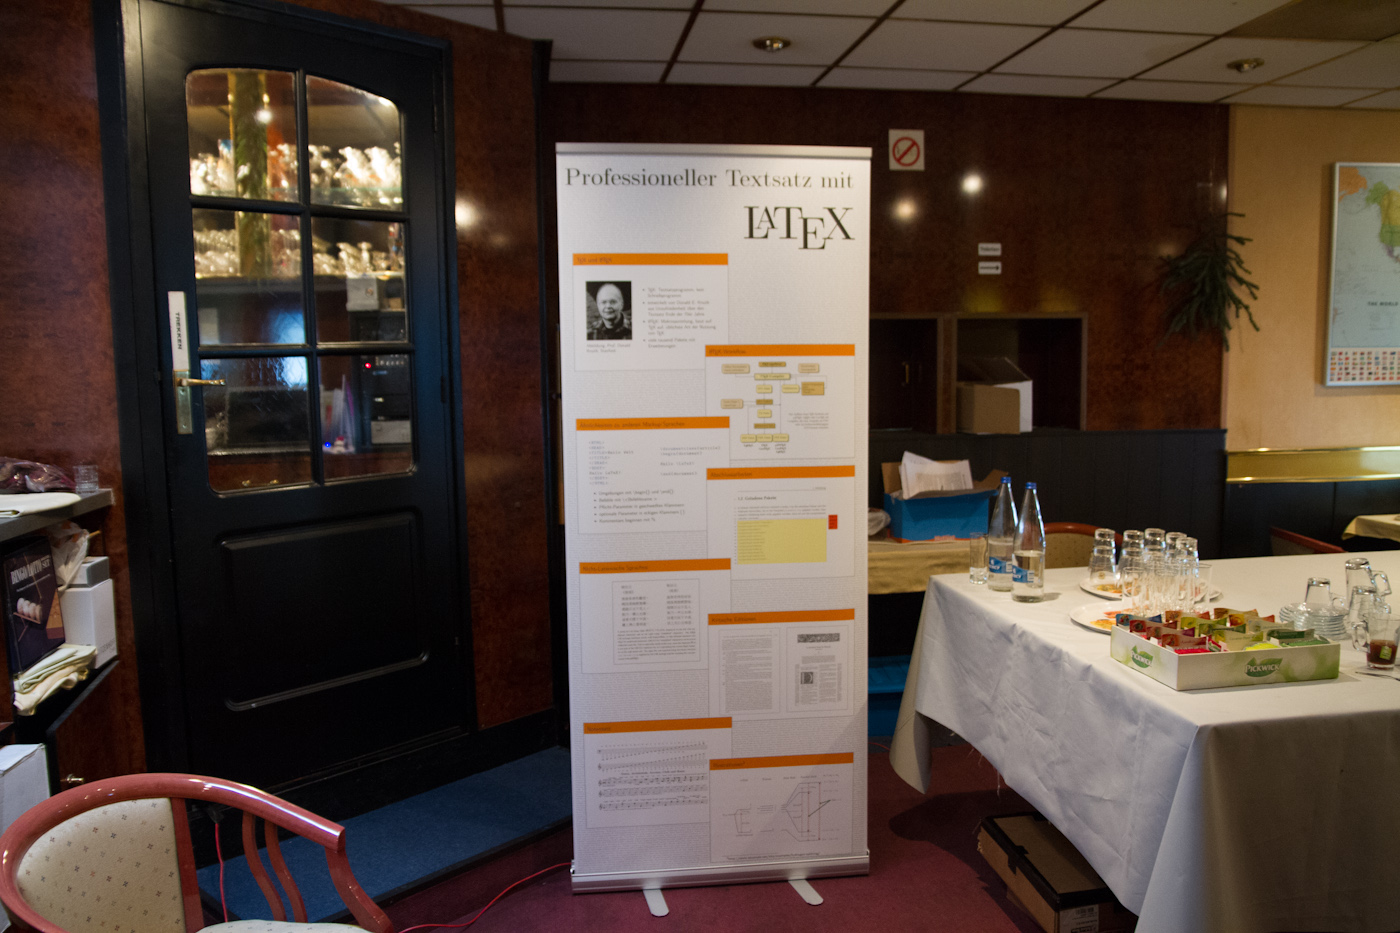
\includegraphics[width=0.9\textwidth]{IMG_2562}
\caption{Foto des fertigen Roll-Up Displays auf der Euro\TeX\ 2012}
\end{figure}




\end{document}


